% !TEX encoding = UTF-8 Unicode
\documentclass[a4paper]{article}

\usepackage{color}
\usepackage{url}
\usepackage[T2A]{fontenc} % enable Cyrillic fonts
\usepackage[utf8]{inputenc} % make weird characters work
\usepackage{graphicx}
\usepackage{amsmath}

\usepackage[english,serbian]{babel}
%\usepackage[english,serbianc]{babel} %ukljuciti babel sa ovim opcijama, umesto gornjim, ukoliko se koristi cirilica

\usepackage[unicode]{hyperref}

\hypersetup{colorlinks,citecolor=green,filecolor=green,linkcolor=blue,urlcolor=blue}

\usepackage{listings}

%\newtheorem{primer}{Пример}[section] %ćirilični primer
\newtheorem{primer}{Primer}[section]

\definecolor{mygreen}{rgb}{0,0.6,0}
\definecolor{mygray}{rgb}{0.5,0.5,0.5}
\definecolor{mymauve}{rgb}{0.58,0,0.82}

\lstset{ 
  backgroundcolor=\color{white},   % choose the background color; you must add \usepackage{color} or \usepackage{xcolor}; should come as last argument
  basicstyle=\scriptsize\ttfamily,        % the size of the fonts that are used for the code
  breakatwhitespace=false,         % sets if automatic breaks should only happen at whitespace
  breaklines=true,                 % sets automatic line breaking
  captionpos=b,                    % sets the caption-position to bottom
  commentstyle=\color{mygreen},    % comment style
  deletekeywords={...},            % if you want to delete keywords from the given language
  escapeinside={\%*}{*)},          % if you want to add LaTeX within your code
  extendedchars=true,              % lets you use non-ASCII characters; for 8-bits encodings only, does not work with UTF-8
  firstnumber=1000,                % start line enumeration with line 1000
  frame=single,                    % adds a frame around the code
  keepspaces=true,                 % keeps spaces in text, useful for keeping indentation of code (possibly needs columns=flexible)
  keywordstyle=\color{blue},       % keyword style
  language=Python,                 % the language of the code
  morekeywords={*,...},            % if you want to add more keywords to the set
  numbers=left,                    % where to put the line-numbers; possible values are (none, left, right)
  numbersep=5pt,                   % how far the line-numbers are from the code
  numberstyle=\tiny\color{mygray}, % the style that is used for the line-numbers
  rulecolor=\color{black},         % if not set, the frame-color may be changed on line-breaks within not-black text (e.g. comments (green here))
  showspaces=false,                % show spaces everywhere adding particular underscores; it overrides 'showstringspaces'
  showstringspaces=false,          % underline spaces within strings only
  showtabs=false,                  % show tabs within strings adding particular underscores
  stepnumber=2,                    % the step between two line-numbers. If it's 1, each line will be numbered
  stringstyle=\color{mymauve},     % string literal style
  tabsize=2,                     % sets default tabsize to 2 spaces
  title=\lstname                   % show the filename of files included with \lstinputlisting; also try caption instead of title
}

\begin{document}

\title{Drugačiji pristup u optimizaciji i primene\\ \small{Seminarski rad u okviru kursa\\Metodologija stručnog i naučnog rada\\ Matematički fakultet}}

\author{Aleksandra Bošković, Stefan Jaćović,\\Milena Stojić, Rajko Jegdić\\ kontakt email aleksandra94@hotmail.rs, stefanjacovic25@gmail.com,\\mstojic39@yahoo.com, rajkojegdic@yahoo.com}

%\date{9.~april 2015.}

\maketitle

\abstract{
U ovom radu ćemo videti kako jedna tehnika iz svakodnevnog života može da se (algoritamski) primeni u problemima optimizacije. Kakva je njena ideja, implementacija i primena na stvarnim problemima. Takođe i kako njome možemo unaprediti već dobro poznate metaheuristike.}

\tableofcontents

\newpage

\section{Uvod}
\subsection{Nastanak}
\label

\textbf{Simulirano kaljenje} (eng. \textit{Simulated Annealing}, SA) je metoda zasnovana na lokalnom pretraživanju, uz mehanizam inspirisan procesom kaljenja čelika koji omogućava izlazak iz lokalnog optimuma. Algoritam je predložen 1983. godine od strane Kirkpatrika i drugih.\cite{sa_history_book}
\subsection{Opis metode}
Pri procesu metalurškog kaljenja čelika cilj je oplemenjivanje metala tako da on postane čvršći. Da bi se postigla čvrstoća metala potrebno je njegovu kristalnu rešetku pomeriti tako da ima minimalnu potencijalnu energiju. Prvi korak u kaljenju čelika je zagrevanje do
određene visoke temperature, a zatim nakon kratkog zadržavanja na toj temperaturu počinje postepeno hlađenje. Pri postepenom hlađenju atomi metala nakon procesa kaljenja formiraju
pravilnu kristalnu rešetku i time se postiže energetski minimum kristalne rešetke. Važno je napomenuti da brzo hlađenje može da uzrokuje pucanje metala.

\begin{figure}[h!]
\centering
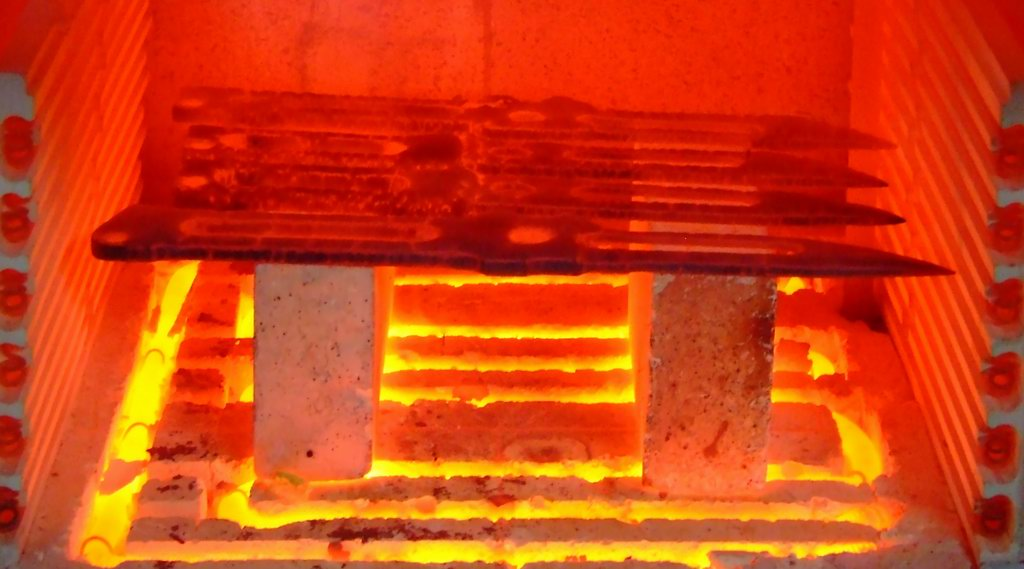
\includegraphics[scale=0.3]{kal.jpg}
\caption{Kaljenje čelika}
\label{fig:universe}
\end{figure}
\subsection{Funkcija cilja}
Funkcija cilja za koju se traži globalni optimum se može posmatrati kao energija kristalne rešetke ako je potrebno minimizovati funkciju cilja ili negativna energija kristalne rešetke ako
je potrebno maksimizovati funkciju cilja. Metoda počinje izborom početnog rešenja i postavljanjem početne temperature na relativno visoku vrednost. Zatim se na slučajan način bira
jedno rešenje iz okoline tekućeg rešenja. Ako je to rešenje bolje, onda ono postaje novo tekuće rešenje. Ako je novo rešenje lošije od tekućeg, ono ipak može da postane tekuće rešenje, ali
sa određenom verovatnoćom. Verovatnoća prihvatanja lošijeg rešenja obično zavisi od parametra koji predstavlja temperaturu i vremenom opada kako se algoritam izvršava. Ovakav pristup obezbeđuje izlazak iz lokalnog optimuma. U početku je ta verovatnoća velika, pa će
u cilju prevazilaženja lokalnog optimuma lošije rešenje biti prihvaćeno. Pred kraj izvršavanja
algoritma verovatnoća prihvatanja lošijeg rešenja je jako mala i to se verovatno neće ni desiti,
jer se smatra da je optimum dostignut ili se nalazi blizu najboljeg posećenog rešenja, pa se
izbegava pogoršanje tekućeg rešenja.


\section{Algoritam}
Ideja implementacije algoritma\cite{sannealingbook} simuliranog kaljenja je sledeća. U svakoj iteraciji algoritma primenjenog na diskretan problem poredimo dve vrednosti rešenja, trenutno najbolje i novo generisano rešenje. Zavisno od uslova odabira između ova dva rešenja za narednu iteraciju dobijeno rešenje prelazi u sledeću iteraciju. Proces ponavljamo  dok god se nezadovolji uslov zaustavljanja. Uslov zaustavljanja moze biti zadat konačnim brojem iteracija ili dok se ne dostigne traženi minimum(maksimum).

\subsection{Definisanje termina}
Da bismo opisali specifičnosti algoritma simuliranog kaljenja, uvedimo nekoliko pojmova, koji će nam biti potrebni za razumevanje samog algoritma. Neka je $\Omega$ prostor mogućih rešenja,$f:\Omega \rightarrow \Re$ funkcija definisana nad prostorom $\Omega$. Cilj je pronaći  $w\in\Omega$ za koje funkcija $f$ doseže minimum(maksimum) problema na koji primenjujemo algoritam simuliranog kaljenja. Ukoliko postoji $w^*\in\Omega$ za koje  važi:$$f(w^*)\geq f(w),\hspace{0.1cm} \forall w \in \Omega$$ tada je $w^*$ traženi maksimum. Da bi ovakvo $w$ postojalo neophodan uslov je da funkcija $f$ bude ograničena na prostoru $\Omega$. Definišimo i funkciju $N(w)$ pomoću koje ćemo određivati susedna rešenja rešenju  $w\in\Omega$ u svakoj iteraciji algoritma pretrage novog rešenja. \par

\subsection{Odabir rešenja}
Neka je $w\in\Omega$ inicijalno rešenje problema koje proizvoljno biramo iz skupa $\Omega$ i $w'\in N(w)$ proizvoljno odabrano susedno rešenje nekim predefinisanim pravilom ili slučajnim izborom. Ukoliko pogledamo uslov da rešenje bude maksimum zaključujemo da nam je bolje ono rešenje koje ima veću vrednost funkcije $f$. Ukoliko bismo u svakoj iteraciji birali rešenje koje ima veću vrednost funkcije $f$ algoritam bi se sveo na algoritam penjanja uzbrdo. Problem algoritma penjanja uzbrdo se javlja kada se naiđe na lokalni maksimum i tu se dalja pretraga zaglavljuje jer svako susedno rešenje nije bolje od njega. Još jedna situacija u kojoj algoritam penjanja uzbrdo pokazuje slabosti je pojava platoa gde iz istog razloga pretraga ostane zaglavljena.Da bismo rešili ovakve probleme algoritam simuliranog kaljenja za odluku koje od dva rešenja će uzeti za sledeću iteraciju bazira na verovatnoći $p$ prihvatljivosti da novo rešenje bude uzeto za trenutno u narednoj iteraciji.
\[ p =
  \begin{cases}
    \exp(f(w')-f(w)/t_k)  \quad f(w) > f(w'),\\
    1  \quad f(w) \leq f(w')\\
  \end{cases}
\]


gde je $t_k$ temperaturni parametar iteracije k i n maximali broj iteracija za koji važi:
$$\forall k\leq n, \quad t_k > 0 \quad \lim_{k \to \infty}t_k=0 $$

\subsection{Implementacija algoritma}
\textbf{Ulaz:} \hspace{0.1cm} Inicijalno rešenje $w$,početna vrednost $t_k$ kao i vrednost $M_k$ koja predstavlja koliko puta ponavljati iteraciju sa datom vrednosću $t_k$
 \par
\textbf{Izlaz:}\hspace{0.1cm} $w$ najbolje rešenje datog problema koje je algoritam uspeo da pronađe
\newline
Ponavljaj:
\begin{itemize}
\item[] $m=0$
\item[]  Ponavljaj:
\begin{itemize}
\item[] generiši novo rešenje  $w'\in N(w)$
\item[] izračunaj vrednost  $\Delta=f(w')-f(w)$
\item[] ako je $\Delta \geq 0$
\begin{itemize}
\item[] $w=w'$ 
\end{itemize}
\item[]inače
\begin{itemize}
\item[] sa verovatnoćom $p=\exp(-\Delta/t_k)$ važi $w=w'$ 
\end{itemize}
\item[]$m=m+1$
\end{itemize}
\item[]dok ne bude $ m=M_k$
\item[] $k=k+1$
\end{itemize}
Dokle god nije zadovoljen uslov zaustavljanja


\subsection{Primena algoritma simuliranog kaljenja\cite{sannealing_tsp_application} na problem trgovačkog putnika}


  Problem trgovačkog putnika je jedan od najizučavanijih kombinatornih problema kao i NP problema. Problem je definisan na sledeći način.
  Data nam je lista gradova koje bi trebalo putnik da obiđe i da se vrati u grad iz kog je pošao. Takođe nam je potreban podatak koja je udaljenost između svaka dva grada iz liste gradova. Naš zadatak je da pronađemo redosled obilaska gradova tako da ukupna dužina puta koji bi trebalo putnik da pređe bude minimalna.\par
  Prvo rešenje koje se nameće je agoritam grube sile, a to je ispitivanje svih mogućih načina obilazaka gradova i odabir najbolje kombinacije za koju je ukupna dužina minimalna. Ovakvo rešenje nije isplativo zbog velike vremenske složenosti koja iznosi n! pri čemu je n broj gradova koje bi trebalo putnik da poseti.\par
    
Da bi problem rešili algoritmom simuliranog kaljenja definišimo prvo šta nam predstavlja temperatura iz ovog algoritma. Temperatura kod ovog problema predstavljala bi meru slučajnosti promene putanje pri čemu se trazi najmanja putanja. Ukoliko je vrednost temperature visoka prave se i veće slučajne promene i pritom se izbegava rizik da ostanemo zaglavljeni u lokalnom optimumu, a njih ima mnogo u posmatranom problemu. Kako temperatura pada tako se spuštamo u skoro optimalni minimum. U svakom koraku kada je potrebna promena temperature njena vrednost je 0.9 puta veća od prethodne. Ovim zadovoljavamo uslov da pad temperature teži nuli kroz rast broja iteracija.\par

Proces kaljenja počinje stazom koja jednostavno navodi sve gradove redosledom njihovog odabira za obilazak. Na svakom temperaturnom koraku se vrši određeni broj slučajnih transformacija puta. Način transformacije puta moze biti različit. Moguće je izabrati dva grada i zameniti njihovo mesto u redosledu obilaska gradova, drugi od nacina bio bi odabrati dve pozicje koje oznacavaju segment koji će se prebaciti na određeno mesto u stazi koja predstavlja redosled obilaska, ili dati segment rotirati. Ukoliko želimo da se vrši više načina transformacija uvodimo \emph{softverski novčić} koji bi određivao vrstu transformacije. 
 Dužina modifikovanog puta se zatim izračunava i upoređuje sa stazom pre modifikacije, stvarajući veličinu koju nazivamo razliku u troškovima. Ako je ta veličina negativna, onda modifikovana putanja je kraća od originalne putanje i uvek je zamenjuje. Međutim, ako dođe do povećanja troškova, eksponencija njegove negativne veličine deljenja sa trenutnom temperaturom upoređuje se sa jednolično raspodeljenim slučajnim brojem između 0 i 1, a ako je veće modifikovana putanja će se koristi iako je povećala troškove. U početku će prihvatanje dužeg puta biti više verovatno jer je temperatura visoka, ali kako temperatura opada biće prihvaćena samo manja povećanja troškova. Broj promena koje se testiraju na svakoj temperaturi je proizvoljan, temperatura se smanjuje i pretraga nastavlja. Nakon isprobavanja svih mogućih scenarija na određenoj temperaturi, nisu pronađene promene koje smanjuju dužinu puta, rešenje se smatra dovoljno dobrim i prikazuje se dobijena staza.

\begin{primer}
Neka nam je dato 5 gradova i matrica M koja predstavlja međusobne udaljenosti između gradova tako da je $M[i][j]$ udaljenost između gradova \textbf{i} i \textbf{j}. Pronaći permutaciju gradova tako da polazeći iz prvog grada se preko ostalih gradova stigne u početni uz uslov da je pređeni put minimalni.\par
Način implementacije rešenja u jeziku Python prikazan je kroz listing \ref{simple}. 
\end{primer}

\begin{lstlisting}[caption={Rešavanje problema TSP korišćenjem SA algoritma},frame=single, label=simple]
import numpy as np
import itertools as per
import random
import math 
M = np.array([
   [0,10,3,12,7],
   [10,0,11,7,3],
   [3,11,0,8,8],
   [12,7,8,0,1],
   [7,3,8,1,0]])
def suma (l):
  return M[l[0]][l[1]]+M[l[1]][l[2]]+M[l[2]][l[3]]+M[l[3]][l[4]]+M[l[4]][l[0]]
Oznake_gradova = np.array([1,2,3,4])
#Postavimo pocetnu permutaciju, tekucu duzinu puta i pocetnu temperaturu
#Pretpostavimo da racunamo jednu iteraciju za svaku temperaturu
minimum=sum(Oznake_gradova)
minimum_perm=Oznake_gradova
t=20
k=0
lista=minimum_perm

while k<7:
  nova_per = random.choices(Oznake_gradova,k=2)
  lista[nova_per[0]], lista[nova_per[1]] = lista[nova_per[1]], lista[nova_per[0]]
  s=suma(lista)
  razlika=s-minimum
  
  if razlika < 0:
    minimum=s
    per_min=lista
  else:
    p=math.exp(-(s-minimum)/t)
    q=random.uniform(0, 1)
    if p > q :
      minimum=s
      per_min=lista
  k=k+1
  t=t*0.9
\end{lstlisting}






\section{Poboljšanje algoritma}

\subsection{Prednosti i nedostaci simuliranog kaljenja}
Prednost simuliranog kaljenja (u odnosu na klasičan genetski algoritam) je dobra lokalna pretraga.\cite{ga_vs_sa_tech_report, gannealingthesis} Ono će uvek naći najbolje rešenje u neposrednoj blizini. Međutim, to je u isto vreme i slabost, iako u teoriji ovaj algoritam može da konvergira ka globalnom optimalnom rešenju.\cite{gannealingthesis} \par
Ovaj nedostatak može da se prevaziđe sa više zasebnih izvršavanja. Svako sledeće izvršavanje počinjemo sa novim početnim rešenjem. Na kraju uzimamo najbolji finalni rezultat. U narednim iteracijama ne koristimo znanje dobijeno u prethodnim iteracijama. To je mana ovog pristupa. \par
Prednost genetskog algoritma u odnosu na simulirano kaljenje je i u višestrukosti rešenja.\cite{gannealingthesis} Simuliranim kaljenjem mi samo poboljšavamo jedno rešenje. Bolja je pretraga zasnovana na $m$ > 1 dobrih rešenja.

\subsection{Genetsko kaljenje}

Dve osnovne metaheuristike koje pripadaju široj grupi algoritama pretage su simulirano kaljenje i genetski algoritam. Sa idejom da se iskoriste prednosti obe metoda nastaje genetsko kaljenje.\cite{gk_master_rad} Tvorac koncepta je Kenneth Price koji je 1994. u svom članku u časopisu \emph{Dr.Bobbs Journal} prvi put izneo ideju o spajanju simuliranog kaljenja i genetskog algoritma. \par
Simulirano kaljenje je algoritam koji se uglavnom primenjuje kada postoji jedno optimalno rešenje, dok se genetski primenjuje u slučaju postojanja više optimalnih rešenja. Ovu ideju koristimo u algoritmu genetskog kaljenja. \par
Genetski algoritam kroz iteracije evoluira ka boljim rešenjima od početno zadatih resenja. U svakoj iteraciji neophodno je odabrati jedinke za ukrštanje i mutaciju. Algoritam genetskog kaljenja ideju simuliranog kaljenja koristi u procesu odabira jedinki.
\newline
\begin{itemize}
\item[]Nasumično odabrati populatiju od N čestica
\item[] brojač iteracija = 0
\item[]  Ponavljaj dok uslov zaustavljanja nije zadovoljen:
\begin{itemize}
\item[] prag = slobodna energija / N
\item[] slobodna energija = 0
\item[] za svaku česticu uradi sledeće:
\begin{itemize}
\item[] mutant = mutiraj
\item[] Ako energija(mutant) < energija(čestica) + prag
\begin{itemize}
\item[]razlika = energija(čestica) + prag - energija(mutant)
\item[]slobodna energija = slobodna energija + razlika
\item[]čestica = mutant
\end{itemize}
\item[]inače 
\begin{itemize}
\item[] slobodna energija = slobodna energija + prag
\end{itemize}
\end{itemize}
\item[]brojac iteracija = brojac iteracija + 1
\item[]slobodna energija = slobodna energija * C
\end{itemize}
\item[]resenje = najbolja(čestica)
\end{itemize}


\subsection{Eksperimentalni rezultati}

U ovom poglavlju ćemo prikazati rezultate primene genetskog kaljenja i uporediti ih sa rezultatima dobijenih simuliranim kaljenjem i genetskim algoritmom. Primeri će nam biti problem trgovačkog putnika i lokacijski problem rutiranja inventara. Cilj je da pokažemo da je hibridizovani pristup bolji od obe zasebne metaheuristike.   \\ 


\subsubsection{Problem trgovačkog putnika (TSP) \cite{gannealingthesis}}

Broj gradova na kome testiramo će biti 40. Kod genetskog kaljenja broj jedinki početne populacije će biti 5, dok će u svakoj narednoj generaciji broj jedinki biti 8. Broj uzastopnih izvršavanja simuliranog kaljenja će biti 40. Maksimalan broj iteracija za oba algoritma će biti 2400. Rezultati dobijeni na 10 različitih primera su prikazani u tabeli \ref{table:1}. \\ 

Iz prikazanog možemo videti da smo u većini slučajeva unapređenom varijantom dobili bolje rezultate. Ovde su izuzetak bili 6. i 8. primer. Kod 6. smo dobili identične rezultate, dok je u 8. primeru simulirano kaljenje dalo bolji rezultat.

\begin{table}[ht]
\begin{center}
\begin{tabular}{|c|c|c|} \hline
     No & Genetsko kaljenje & Simulirano kaljenje  \\ \hline
     1 &  3180 & 3360 \\ \hline
     2 &  2900 & 3020 \\ \hline
     3 &  3040 & 3100 \\ \hline
     4 &  3120 & 3460 \\ \hline
     5 &  2300 & 2460 \\ \hline
     6 &  3100 & 3100 \\ \hline
     7 &  2420 & 2720 \\ \hline
     8 &  2400 & 2080 \\ \hline
     9 &  3220 & 3300 \\ \hline
     10 & 3040 & 3120 \\ \hline
\end{tabular}
\end{center}
\label{table:1}
\caption{Dobijeni rezultati na problemu trgovačkog putnika}
\end{table}

\subsubsection{Lokacijski problem rutiranja inventara (eng. \textit{Location-Inventory-Routing Problem}, LIRP) \cite{gannealingaplication}}

\large{Opis problema}  \normalsize

Lanac elektronske trgovine čine proizvođač, skladišta i prodajni objekti. Proizvođač šalje robu skladištima, a iz njih se šalje u prodajne objekte. U prodajnim objektima se roba prodaje ili putuje dalje u naredni prodajni objekat. Iz nekog od njih ako se ne proda se vraća nazad u skladište iz kog je krenula. Roba koja se vraća je obično u dobrom stanju i posle samog prepakovanja može ponovo da se vrati u prodaju. 

\begin{figure}[h!]
\centering
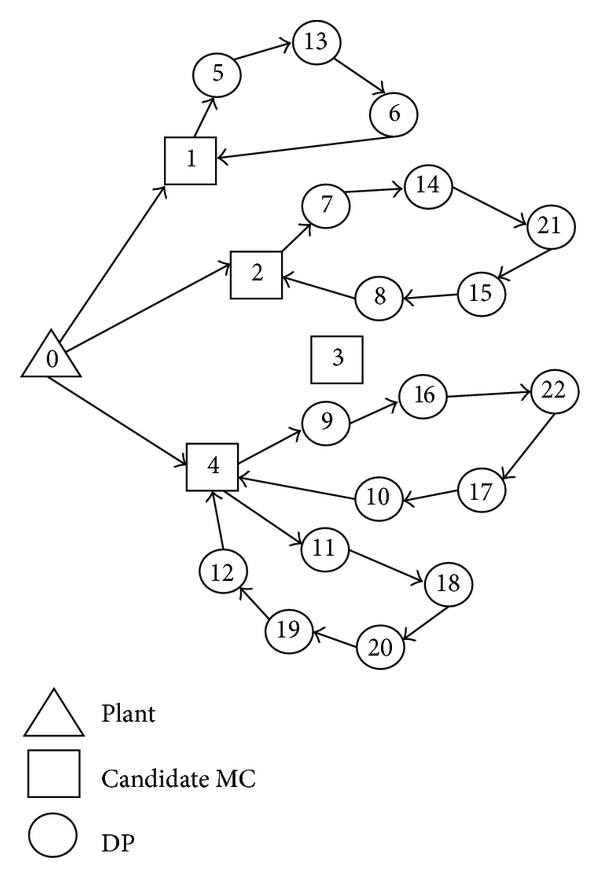
\includegraphics[scale=0.25]{LIRP_Primer_Grafa.jpg}
\caption{Primer mreže lanca e-trgovine}
\label{fig:2}
\end{figure}
\newpage
Primer jedne mreže ovog lanca trgovine se nalazi na slici \ref{fig:2}. Čvor u obliku trougla predstavlja proizvođača, kvadrati su skladišta, a krugovi prodajna mesta. U ovom problemu imamo samo jednog proizvođača. \par
Poznate su nam lokacije proizvođača, prodajnih mesta, svih potencijalnih skladišta (ne moramo sve da ih uključimo u lanac), troškovi transporta između svaka dva čvora i svi ostali troškovi. Naš zadatak je da odredimo optimalan broj i lokacije skladišta kao i rute od skladišta do prodajnih objekata tako da troškovi budu što manji. \par
Na ovom problemu ćemo prikazati rezultate dobijene primenom genetskog kaljenja i klasičnog genetskog algoritma. \\  \par

Funkcija cilja su ukupni troškovi i nju minimizujemo. U oba algoritma se u implementaciji koristi ruletska selekcija, a funkcija prilagođenosti je obrnuto srazmerna funkciji cilja. Implementirani su u programskom jeziku Matlab. \\ \par
Algoritam je testiran na podacima \textit{Gaskell 67-29x5} iz LIRP baze podataka sa Univerziteta Aveira \cite{lrp_database}. Kao što se iz samog naziva skupa podataka može videti, radi se o instanci problema gde imamo 29 prodajnih mesta i 5 potencijalnih skladišta. 

\begin{figure}[h!]
\centering
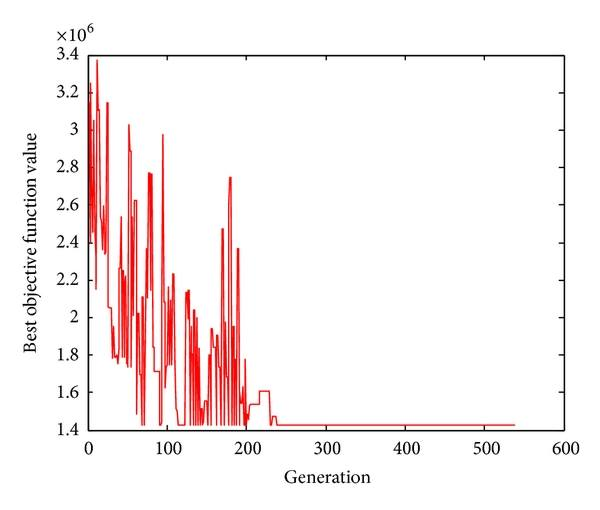
\includegraphics[scale= 0.4]{LIRP_Grafik_Genetsko_Kaljenje.jpg}
\caption{Najmanja vrednost funkcije cilja u svakoj generaciji, genetsko kaljenje}
\label{fig:3}
\end{figure}

Na slici \ref{fig:3} se mogu videti najmanje vrednosti funkcije cilja u svakoj generaciji za algoritam genetsko kaljenje, a na slici \ref{fig:4} za genetski algoritam.

\newpage
\begin{figure}[h!]
\centering
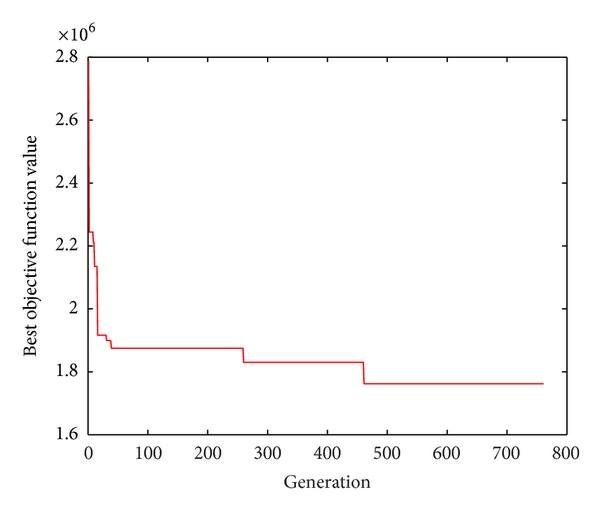
\includegraphics[scale= 0.4]{LIRP_Grafik_Genetski_Algoritam}
\caption{Najmanja vrednost funkcije cilja u svakoj generaciji, genetski algoritam}

\label{fig:4}centering
\end{figure}

Kod genetskog kaljenja u prvih 200 generacija imamo velika oscilovanja optimalnog rešenja. Posle se ubrzo dolazi do optimuma koji se ne menja do zaustavljanja. Uz ukupan manji broj iteracija se dolazi do manje vrednosti funkcije cilja nego genetskim algoritmom.

U tabeli \ref{table:2} se mogu videti i statistike najmanjih vrednosti funkcije cilja u svim generacijama. One su takođe na strani genetskog kaljenja. Čak je i standardna devijacija znatno manja kod genetskog kaljenja, bez obzira na početna oscilovanja.

\begin{table}[ht]
\centering
\resizebox{\columnwidth}{!}{%
\begin{tabular}{|l|c|c|c|c|} \hline
     Algoritam & Najveća vrednost & Najmanja vrednost & Srednja vrednost & Standardna devijacija \\ \hline
     Genetsko kaljenje &  1989900.00 & 1078700.00 & 1605543.33	& 262462.64 \\ \hline
     Genetski algoritam & 2410900.00 & 1142000.00 & 1644678.00 & 353993.10 \\ \hline
\end{tabular}
}
\label{table:2}
\caption{Statistike najmanjih vrednosti funkcije cilja u svim generacijama}
\end{table}

Isti eksperimenti su takođe pokazali da je i procesorsko vreme izvršavanja manje kod genetskog kaljenja. Dakle, osim što ovaj algoritam daje bolja rešenja, pokazalo se i da je računski efikasnije. \par Vršeni su i dalji obimniji eksperimenti na ovom problemu\cite{gannealingaplication} (na istoj LIRP bazi podataka) koji su samo potvrdili sve dobijene zaključke.


\section{Zaključak}
\label{sec:zakljucak}

Pojava metode \textbf{simuliranog kaljenja} je napravila veliki pomak u teoriji optimizacije. Sama metaheuristika (u više ciklusa) pronalazi veoma dobra rešenja. Međutim, pokazuje se \cite{gannealingthesis, gannealingaplication} da su poboljšanja svih ostalih algoritama umetanjem koncepta simuliranog kaljenja još značajnija. Time nastaju veoma moćni algoritmi.


\newpage
\addcontentsline{toc}{section}{Literatura}

\appendix

\bibliography{seminarski}
\bibliographystyle{plain}
\nocite{*}

\end{document}